\documentclass[11pt]{article}
\usepackage[margin=1in, top=1in]{geometry}
\usepackage[all]{nowidow}
\usepackage[hyperfigures=true, hidelinks, pdfhighlight=/N]{hyperref}
\usepackage[separate-uncertainty=true, group-digits=false]{siunitx}
\usepackage{graphicx,amsmath,physics,tabto,float,amssymb,pgfplots,verbatim,tcolorbox}
\usepackage{listings,xcolor,subfig,caption,import,wrapfig}
\usepackage[version=4]{mhchem}
\usepackage[noabbrev]{cleveref}
\newcommand{\creflastconjunction}{, and\nobreakspace}
\numberwithin{equation}{section}
\numberwithin{figure}{section}
\numberwithin{table}{section}
\definecolor{stringcolor}{HTML}{C792EA}
\definecolor{codeblue}{HTML}{2162DB}
\definecolor{commentcolor}{HTML}{4A6E46}
\captionsetup{font=small, belowskip=0pt}
\lstdefinestyle{appendix}{
    basicstyle=\ttfamily\footnotesize,commentstyle=\color{commentcolor},keywordstyle=\color{codeblue},
    stringstyle=\color{stringcolor},showstringspaces=false,numbers=left,upquote=true,captionpos=t,
    abovecaptionskip=12pt,belowcaptionskip=12pt,language=Python,breaklines=true,frame=single}
\lstdefinestyle{inline}{
    basicstyle=\ttfamily\footnotesize,commentstyle=\color{commentcolor},keywordstyle=\color{codeblue},
    stringstyle=\color{stringcolor},showstringspaces=false,numbers=left,upquote=true,frame=tb,
    captionpos=b,language=Python}
\renewcommand{\lstlistingname}{Appendix}
\pgfplotsset{compat=1.17}

\begin{document}

\begin{center}
    {\huge Parametrically driven, damped nonlinear Schr\"odinger equation}\\
    \vspace{0.2in}
    \textbf{KDSMIL001 | October 2021}

    \begin{abstract}
        We find the region of stability for a parametrically driven, damped nonlinear Schr\"odinger equation, find the conditions for an exact soliton solution, and then simulate the equation using the split step Fourier method.
    \end{abstract}
    
\end{center}

\section{Introduction}\label{sec:Introduction}
\par The equation of interest to us is the following:
\begin{equation}
    i\psi_t+\psi_{xx}+2|\psi|^2\psi-\psi=h\psi^*-i\gamma\psi=0
    \label{eqn:original}
\end{equation}
Here $\gamma>0$ is the damping coefficient and $h>0$ is the amplitude of the driving term. 

\section{Finding the dispersion relation}\label{sec:Dispersion}
\par To begin, since $\psi$ is a complex number, let us express it in terms of its components, letting 
\begin{equation}
    \psi = u+iv\;\;\implies\;\; \psi^*=u-iv
\end{equation}
where $u$ and $v$ are both real numbers. Doing this, we are able to re-express \cref{eqn:original} in this form, leading to
\begin{equation}
    iu_t-v_t+u_{xx}+iv_{xx}+2(u^2+v^2)(u+iv)-u-iv=hu-hiv-i\gamma u+\gamma v=0
    \label{eqn:expanded original}
\end{equation}
\par This has very neatly handled the problem of the complex conjugate, as otherwise that would've been a nasty guy to try and tackle. The other problem we have with this equation is the nonlinear part, stemming from the $2|\psi|^2\psi$ term in \cref{eqn:original}. As we are seeking a dispersion relation and nonlinearity tends to rain on the parade of dispersion relations, we will simply let this term wander off into the night, never to be seen again. This can be done if we are considering small values of $u$ and $v$. (This translates into small amplitude waves when we make the substitution in \cref{eqn:u wave,eqn:v wave}, but let's not get ahead of ourselves.)
\par Since this \cref{eqn:expanded original} is equal to zero, both its real and imaginary parts must be equal to zero, handily leading us to two separate, but coupled, equations. 
\begin{align}
    (\partial_{xx}-1-h)u+(-\partial_t-\gamma)v&=0\\
    (\partial_t+\gamma)u+(\partial_{xx}-1+h)v&=0
\end{align}
\par These are a pair of coupled Schr\"odinger equations and we know what kind of solution Schr\"odinger equations have: travelling waves. Let us guess two waves for $u$ and $v$ and see what happens:
\begin{align}
    u&=Ue^{i(\omega t-kx)}\label{eqn:u wave}\\
    v&=Ve^{i(\omega t-kx)}\label{eqn:v wave}
\end{align}
\par Substituting these back into our coupled equations, and noting that space derivatives will yield simply $-ik$ and time derivatives will yield $-\omega$, we find
\begin{align*}
    (-k^2-1-h)Ue^{i(\omega t-kx)}+(i\omega-\gamma)Ve^{i(\omega t-kx)}&=0\\
    (i\omega+\gamma)Ue^{i(\omega t-kx)}+(-k^2-1+h)Ve^{i(\omega t-kx)}&=0
\end{align*}
\par Thankfully, we can divide through both equations by the exponential, leaving us with a simple algebraic system of equations with unknowns $U$ and $V$
\begin{align*}
    -(k^2+1+h)U-(i\omega+\gamma)V&=0\\
    (i\omega+\gamma)U-(k^2+1-h)V&=0
\end{align*}
which can be re-expressed as a matrix equation:
\begin{equation}
    \begin{pmatrix}
        -(k^2+1+h) & -(i\omega+\gamma)\\
        (i\omega+\gamma) & -(k^2+1-h)
    \end{pmatrix}
    \begin{pmatrix}
        U\\
        V
    \end{pmatrix}
    =0
\end{equation}
\par We know from linear algebra that this system of equations has a nontrivial solution only if the determinant of this matrix is zero. So we have 
\begin{align*}
    0&=(k^2+1+h)(k^2+1-h)+(i\omega+\gamma)^2\\
    &=k^4+k^2-k^2h+k^2+1-h+k^2h+h-h^2-\omega^2+2i\omega\gamma+\gamma^2\\
    &=\omega^2-2i\gamma\omega-k^4-2k^2+h^2-\gamma^2-1\\
\end{align*}
\par We can now solve for $\omega$ with the quadratic formula:
\begin{align*}
    \omega&=\frac{2i\gamma\pm\sqrt{(-2i\gamma)^2+4(k^4-2k^2+h^2-\gamma^2-1)}}{2}\\
    &=i\gamma\pm\sqrt{k^4+2k^2-h^2+1}
\end{align*}
where we will label the two branches with $\omega_\pm$.
\begin{equation}
    \omega_\pm=i\gamma\pm\sqrt{k^4+2k^2-h^2+1}
    \label{eqn:dispersion relation}
\end{equation}
\par The dispersion relation of a differential equation can tell us about the stability of the equation. Our ansatz in \cref{eqn:u wave,eqn:v wave} has an exponential. If this exponential has a positive, real value in the exponent, the solution will simply grow. This is instability. If there is a negative real value in the exponent we see stability, and if there is no real part we will see stable oscillations. The dispersion relation we found is for $\omega$ in terms of $k$, $\gamma$, and $h$, and the exponential in our ansatz has an $i\omega t$ term in the exponent. To find stability we must then consider when $\omega$ has a non-negative imaginary component as the $i^2$ will give us a non-positive real term in the exponent.
\par Let us begin by examining the square root in \cref{eqn:dispersion relation}. When $h^2\leq k^4+2k^2+1$, the square root term is real. When $h^2>k^4+2k^2+1$, the term is imaginary and positive.
\par The first branch we will consider is $\omega_+$, which for $h^2\leq k^4+2k^2+1$ has a non-negative imaginary part only when $\gamma\geq0$. For $h^2>k^4+2k^2+1$, the imaginary part is $\gamma+\sqrt{h^2-k^4-2k^2-1}$, which is only non-negative if $\gamma\geq-\sqrt{h^2-k^4-2k^2-1}$. \Cref{fig:stabilityPlus} shows the regions of the $(\gamma, h)$ plane for which \cref{eqn:original} is stable.
\par For the $\omega_-$ branch, again for $h^2\leq k^4+2k^2+1$ the only imaginary part is $\gamma$ and so we have stability for $\gamma\geq0$. For $h^2>k^4+2k^2+1$, the imaginary part is now $\gamma-\sqrt{h^2-k^4-2k^2-1}$, so we have stability for $\gamma\geq\sqrt{h^2-k^4-2k^2-1}$. \Cref{fig:stabilityMinus} shows the regions on the $(\gamma, h)$ plane for which \cref{eqn:original} is stable.

\begin{figure}[H]
    \begin{center}
        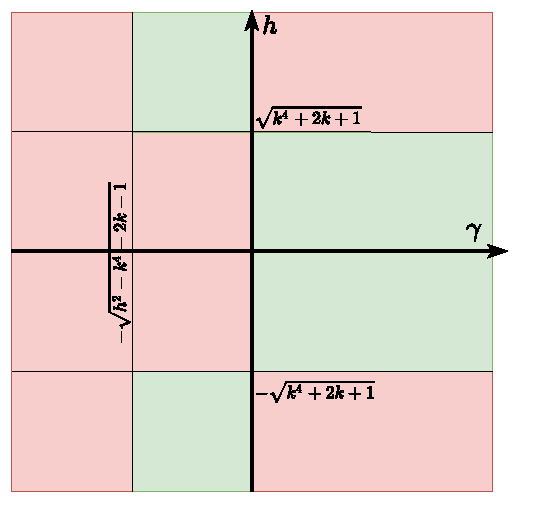
\includegraphics[width=0.5\textwidth]{Plots/stabilityPlus.pdf}
        \caption{Stability diagram for the $\omega_+$ branch. Red means unstable and green means stable.}
        \label{fig:stabilityPlus}
    \end{center}
\end{figure}
\begin{figure}[H]
    \begin{center}
        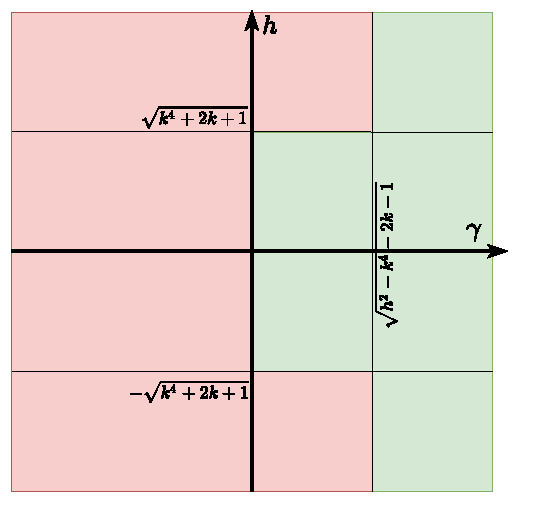
\includegraphics[width=0.5\textwidth]{Plots/stabilityMinus.pdf}
        \caption{Stability diagram for the $\omega_-$ branch. Red means unstable and green means stable.}
        \label{fig:stabilityMinus}
    \end{center}
\end{figure}

\section{Verifying an exact soliton solution}\label{sec:soliton solution}
\par We are asked to find the values of $A$ and $\theta$ for which 
\begin{equation}
    \psi(x)=Ae^{-i\theta}\sech(Ax)
    \label{eqn:soliton}
\end{equation}
is an exact soliton solution to \cref{eqn:original}. We can do this simply by substituting the solution in. First we notice that this solution has no time dependence, so its derivative with respect to $t$ is zero. Next we can find its derivatives with respect to $x$:
\begin{align*}
    \psi'(x)&=Ae^{-i\theta}(-\tanh(Ax)A\sech(Ax))\\
    \psi''(x)&=-A^2e^{-i\theta}(\tanh(Ax)(-\tanh(Ax)A\sech(Ax))+\sech(Ax)(A\sech^2(Ax)))\\
    &=A^3e^{-i\theta}\sech(Ax)(\tanh^2(Ax)-\sech^2(Ax))
\end{align*}
And we can also easily see
\begin{equation*}
    |\psi|^2=A^2\sech^2(Ax)
\end{equation*}
Inserting these back into \cref{eqn:original}, we get
\begin{align*}
    0=&A^3e^{-i\theta}\sech(Ax)(\tanh^2(Ax)-\sech^2(Ax))+2A^2\sech^2(Ax)Ae^{-i\theta}\sech(Ax)\\ &-Ae^{-i\theta}\sech(Ax)-hAe^{i\theta}\sech(Ax)+i\gamma Ae^{-i\theta}\sech(Ax)\\
    =&A^3\sec(Ax)\left[\tanh^2(Ax)-\sech^2(Ax)+2\sech^2(Ax)\right]+A\sech(Ax)\left[i\gamma-1-he^{2i\theta}\right]
\end{align*}
where in the last line we have divided through by $e^{-i\theta}$ as it is always positive. The bracket in the first term simplifies to $\tanh^2(Ax)+\sech^2(Ax)=1$, so we get
\begin{align*}
    0&=A^3\sech(Ax)+A\sech(Ax)\left[i\gamma-1-he^{2i\theta}\right]\\
    &=A\sech(Ax)\left[A^2+i\gamma-1-he^{2i\theta}\right]
\end{align*}
Now $\sech(Ax)$ is never zero so long as $x$ is finite, and $A=0$ is just the trivial solution, so we can simplify this further to have
\begin{align*}
    0&=A^2+i\gamma-1-he^{2i\theta}\\
    &=A^2+i\gamma-1-h(\cos(2\theta)+i\sin(2\theta))\\
    &=A^2-1-h\cos(2\theta)+i(\gamma-h\sin(2\theta))
\end{align*}
Since both the real and imaginary parts of the right hand side must be zero, we can split this into two equations:
\begin{equation}
    \begin{aligned}
        0&=A^2-1-h\cos(2\theta)\\
        \implies A&=\pm\sqrt{h\cos(2\theta)+1}
    \end{aligned}
    \qquad\textrm{and}\qquad
    \begin{aligned}
        0&=\gamma-h\sin(2\theta)\\
        \implies \theta&=\frac{\arcsin(\gamma/2)}{2}
    \end{aligned}
    \label{eqn:A theta}
\end{equation}
\par Under these conditions of $A$ and $\theta$, \cref{eqn:soliton} is an exact soliton solution of \cref{eqn:original}. 

\section{Simulation}\label{sec:simulation}
\par The numerical method we chose to use was the split step Fourier method as it works very well for nonlinear Schr\"odinger equations. In our case, the complex conjugate term tripped us up a bit, but \cite{Mariana Bondila} studies precisely the same equation and they use the split step method to simulate the equation, so we have stood firmly on the shoulders of those specific giants in order to investigate \cref{eqn:original} numerically. The details of how to implement this method is outlined on pages 32-40.
\par We implemented the steps outlined by \cite{Mariana Bondila}, considering the stability condition mentioned on page 39, and found \cref{eqn:soliton} to be a stationary soliton for the $A$ and $\theta$ found in \cref{eqn:A theta}.

\begin{figure}[h]
    \begin{center}   
        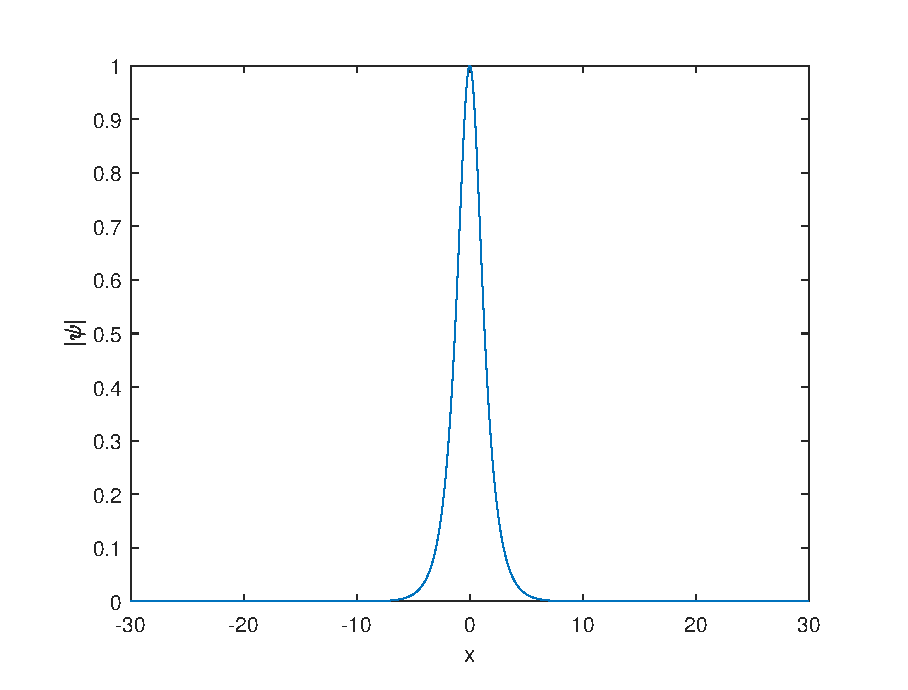
\includegraphics[scale=0.6]{Plots/initialCondition.eps}
        \caption{The initial condition used in the simulation: $\psi=Ae^{-i\theta}\sech(Ax)$, with $A$ and $\theta$ determined from \cref{eqn:A theta}. $\gamma=h=0.25$.}
        \label{fig:initialCondition}
    \end{center}
\end{figure}
\begin{figure}[h]
    \begin{center}
        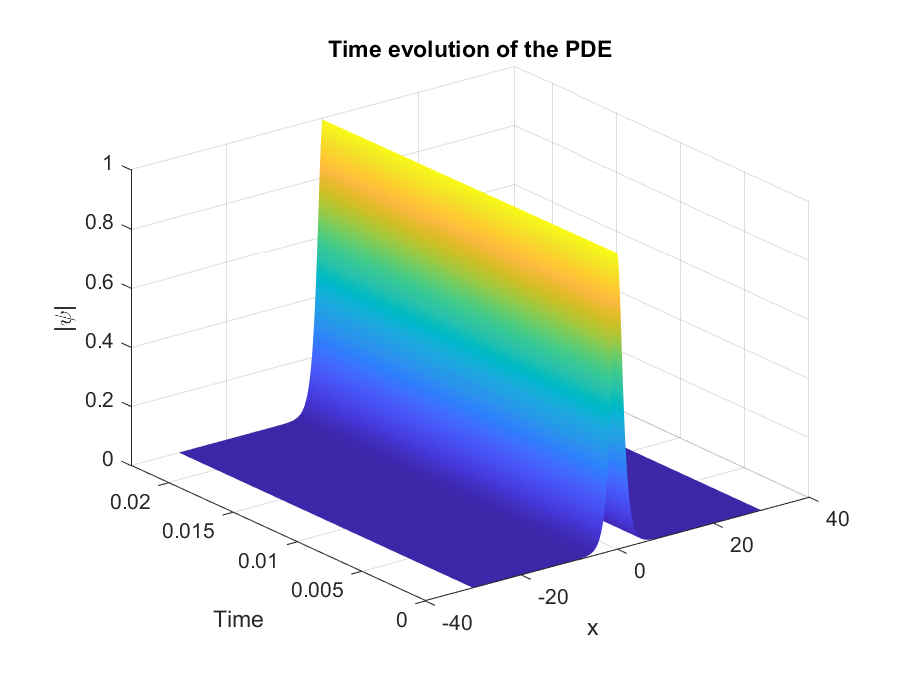
\includegraphics[scale=0.6]{Plots/timeEvolution.eps}
        \caption{Time evolution of \cref{eqn:original}, simulated using split step fourier method. Initial conditions the same as \cref{fig:initialCondition}. Simulation ran for 1000 time steps.}
        \label{fig:timeEvolution}
    \end{center}
\end{figure}
\par \Cref{fig:initialCondition} shows an example of the initial condition used in the following simulations. We kept $\gamma$ fixed at 0.25 and tried various values of $h\in[0.25,1]$ and found there to be no difference in evolution of the state, aside from a difference in height of the soliton, due to the dependence of $A$ and $\theta$ on $h$. In fact we found that the soliton was completely stationary for all time, as can be seen in \cref{fig:timeEvolution}.


\par It makes sense that the soliton is stationary as the initial condition, \cref{eqn:soliton}, has no time dependence. It also makes sense that it remains constant as, given that it's a solution to \cref{eqn:original}, it will always remain a solution.

\section{Conclusion}\label{sec:Conclusion}
\par We found the dispersion relation for \cref{eqn:original}, shown in \cref{eqn:dispersion relation}. From there we were able to find the regions on the $(\gamma,h)$ plane for which the differential equation is stable. This was split into two branches, $\omega_+$ and $\omega_-$. We then found the $A$ and $\theta$ for which \cref{eqn:soliton} is an exact soliton solution to \cref{eqn:original}, which is given in \cref{eqn:A theta}. We simulated \cref{eqn:original} using \cref{eqn:soliton} as an initial condition and found it to be a stationary soliton.



\begin{thebibliography}{9}
    \bibitem{Mariana Bondila}
    M. Bondila, \textit{Numerical study of the parametrically driven damped nonlinear Schr\"odinger equation}, University of Cape Town, (1995)
    
\end{thebibliography}
\end{document}